\chapter{Il Protocollo IPv6}

\section{Motivazioni e cenni storici}

Il protocollo IP versione 4 (IPv4), standardizzato negli anni '80 con indirizzi a 32 bit, è stato progettato in un'epoca in cui Internet collegava principalmente pochi centri universitari. Già a partire dagli anni '90 è emersa la necessità di definire una nuova versione del protocollo. Sebbene siano state proposte diverse motivazioni accessorie (migliore efficienza sulle LAN, supporto nativo a multicast e anycast, sicurezza integrata tramite IPsec, meccanismi plug-and-play e supporto alla Quality of Service), l'unica vera necessità fondamentale che ha spinto l'adozione di IPv6 è l'esaurimento dello spazio di indirizzamento: \textbf{c'è bisogno di uno spazio di indirizzi più grande}.

Tutte le funzionalità aggiuntive introdotte nativamente in IPv6 (come la sicurezza o l'autoconfigurazione) avrebbero potuto essere, e in molti casi lo sono state, implementate in IPv4 tramite protocolli aggiuntivi (si pensi a IPsec o al DHCP).

\subsection{Il problema dell'esaurimento degli indirizzi IPv4}
Con 32 bit, IPv4 mette a disposizione circa 4 miliardi di indirizzi (più precisamente $2^{32}$). Tuttavia, questo numero teorico si riduce drasticamente nella pratica:
\begin{itemize}
    \item \textbf{Allocazione gerarchica e sprechi:} Molti indirizzi sono riservati (es. multicast, classi sperimentali) e molti sono stati sprecati a causa dell'iniziale divisione in classi (A, B, C). Nei primi anni, venivano assegnati interi blocchi \texttt{/8} (Classe A, corrispondenti a milioni di indirizzi) ad aziende che ne utilizzavano solo una minima parte. Poiché un prefisso identifica una specifica rete fisica (subnet), gli indirizzi non utilizzati all'interno di quel prefisso non possono essere riassegnati altrove.
    \item \textbf{Proliferazione dei dispositivi:} Oltre alla popolazione mondiale, bisogna considerare l'avvento di smartphone, tablet e, soprattutto, dell'Internet of Things (IoT). Dispositivi domotici come frigoriferi, forni intelligenti e sistemi di antifurto necessitano oggi di un indirizzo IP, portando il fabbisogno ben oltre i 4 miliardi.
\end{itemize}

Lo IANA (Internet Assigned Numbers Authority) ha esaurito il proprio pool centrale di indirizzi (i blocchi \texttt{/8}) nel febbraio 2011, delegando gli ultimi blocchi ai vari Regional Internet Registry (RIPE NCC per l'Europa, ARIN, APNIC, ecc.), i quali a loro volta stanno esaurendo le scorte.

% FIGURA ORIGINALE DA RECUPERARE DALLE SLIDE
% Slide di provenienza: "IPv4 Address Pool status" e "Current IPv4 Status"
% Tipo: Grafici a barre
% Descrizione: Grafici che mostrano l'esaurimento dei blocchi /8 IANA e la quantità di prefissi annunciati e non annunciati.
% Punto di inserimento: Inizio sezione esaurimento IP.
\begin{figure}[H]
    \centering
    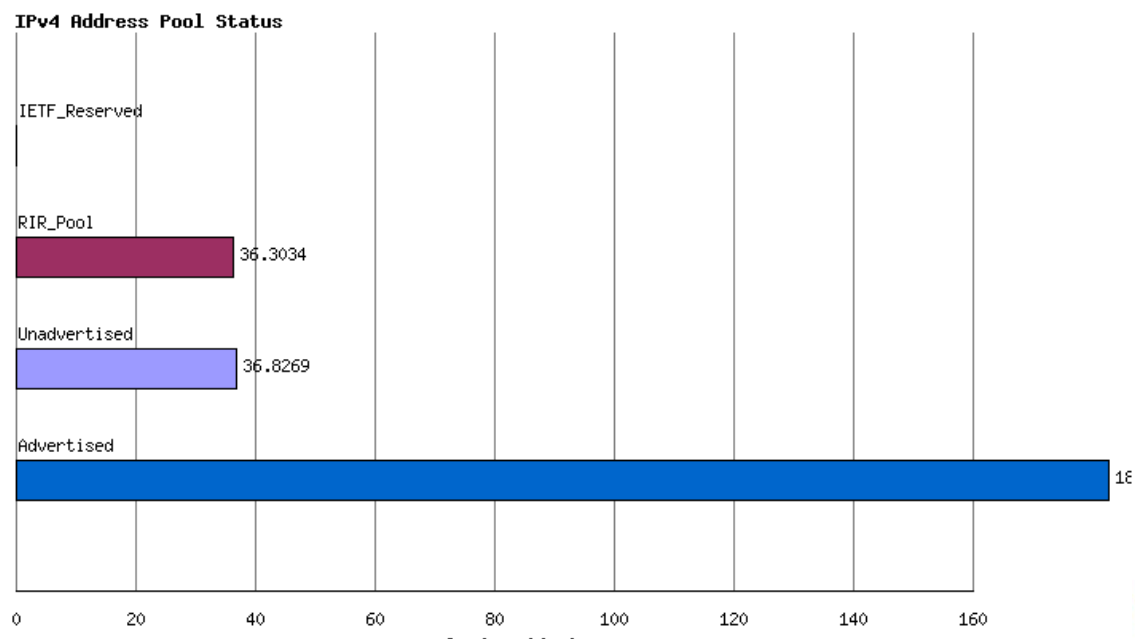
\includegraphics[width=0.7\textwidth]{capitoli/02-IPv6/images/ipv4_pool_status}
    \caption{Stato dell'allocazione dei prefissi IPv4 e progressivo esaurimento dei blocchi IANA.}
    \label{fig:ipv4-pool}
\end{figure}

\subsection{Soluzioni temporanee (Interim solutions) per IPv4}
La transizione a IPv6 si sta rivelando estremamente lunga poiché richiede l'aggiornamento di un protocollo fondamentale nel backbone della rete (modificare l'hardware e i sistemi operativi dei router di base è complesso e costoso). Come analogia, il professore cita il "Dagen H" svedese (quando si invertì il senso di marcia in un solo giorno), un cambiamento drastico impraticabile per Internet, dove la transizione è graduale e senza una data di scadenza definita.

Per posticipare l'esaurimento di IPv4, sono state introdotte delle "toppe":
\begin{itemize}
    \item \textbf{Subnetting flessibile (CIDR):} L'abbandono delle classi a favore delle netmask.
    \item \textbf{Indirizzi privati (RFC 1918) e NAT:} L'introduzione di indirizzi IP privati (es. \texttt{10.0.0.0/8}, \texttt{192.168.0.0/16}) utilizzabili localmente nelle LAN domestiche o aziendali. Poiché questi non sono instradabili su Internet, è stato introdotto il NAT (Network Address Translation). Il NAT mappa gli IP privati di una rete locale su uno o pochi IP pubblici per uscire su Internet. 
\end{itemize}
Sebbene il NAT abbia salvato IPv4, rompe il principio di raggiungibilità end-to-end (end-to-end reachability). Se un host esterno vuole iniziare una comunicazione verso un server situato dietro un NAT domestico, è necessario configurare manualmente il port forwarding, un'operazione complessa, resa a volte impossibile dall'adozione del \textit{Carrier-Grade NAT} (dove il NAT è gestito direttamente dall'ISP, precludendo all'utente il controllo sull'IP pubblico).

\subsection{Il problema della scalabilità del routing}
Un ulteriore motivo fondamentale, oltre alla scarsità di indirizzi, riguarda la dimensione delle tabelle di routing nei router di backbone (BGP tables).
A causa dell'assegnazione non razionale dei prefissi IPv4 avvenuta in passato, non è più possibile aggregare efficacemente le rotte. Di conseguenza, i router centrali di Internet devono memorizzare ed elaborare centinaia di migliaia di entry (oltre 900.000 nel 2023, superando il milione nel 2026), richiedendo hardware costoso e rallentando le operazioni.

% FIGURA ORIGINALE DA RECUPERARE DALLE SLIDE
% Slide di provenienza: "Growth of BGP Tables"
% Tipo: Grafico lineare
% Descrizione: Crescita esponenziale del numero di entry nelle tabelle BGP nei router di backbone dal 1994 a oggi.
% Punto di inserimento: Fine spiegazione della scalabilità del routing.
\begin{figure}[H]
    \centering
    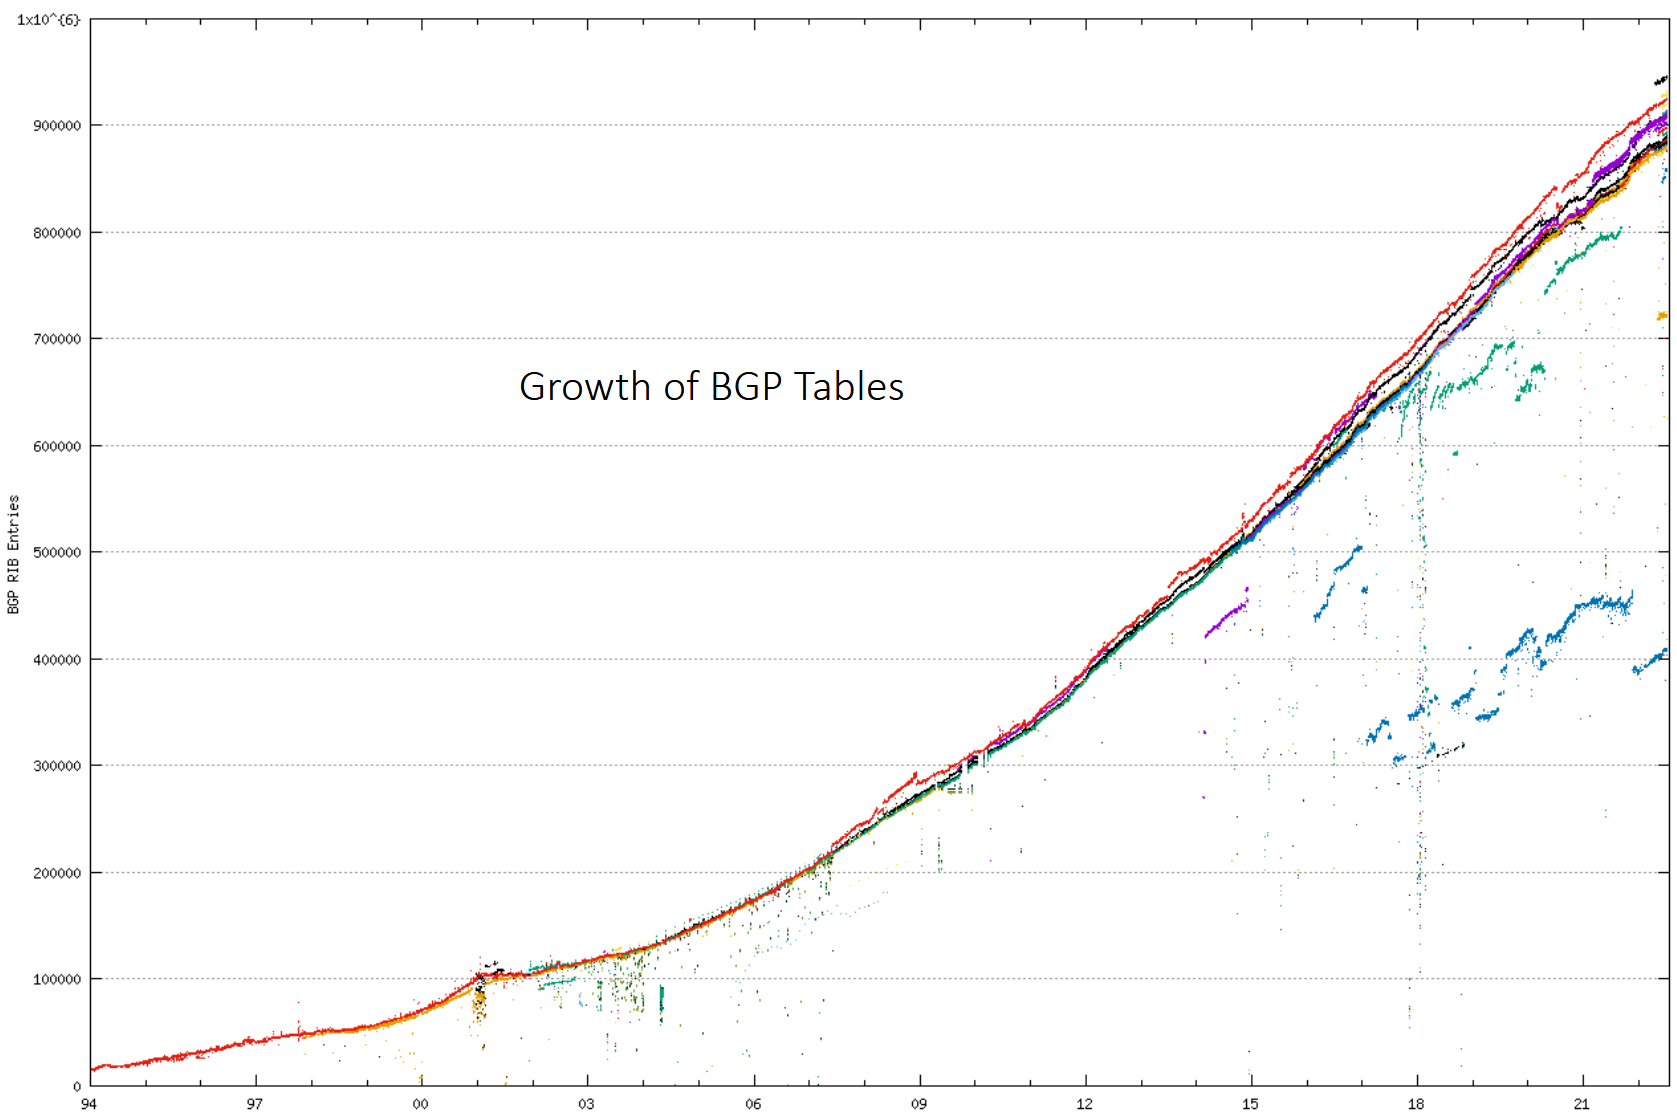
\includegraphics[width=0.85\textwidth]{capitoli/02-IPv6/images/bgp_growth}
    \caption{Crescita delle entry nelle tabelle di routing BGP dovuta alla frammentazione dei prefissi IPv4.}
    \label{fig:bgp-growth}
\end{figure}

\section{Indirizzamento IPv6}

Il gruppo di lavoro IETF ha valutato diverse proposte per il nuovo protocollo (es. TUBA, CATNIP), ma alla fine è stata scelta la proposta \textbf{SIPP} (Simple Internet Protocol Plus), che prevedeva modifiche incrementali rispetto a IPv4, adottando uno spazio di indirizzamento a \textbf{128 bit} (RFC 1883, poi aggiornato nell'RFC 8200). 
Nota: "IPv5" fu assegnato a un protocollo sperimentale che non divenne mai uno standard.

\subsection{Perché 128 bit?}
Sebbene 128 bit generino un numero di combinazioni spropositato ($3,4 \times 10^{38}$), la scelta non è motivata unicamente dalla necessità di fornire un identificativo univoco a ogni dispositivo. Se l'obiettivo fosse stato solo l'identificazione univoca, sarebbero bastati meno bit (i MAC address, ad esempio, sono univoci a livello globale utilizzando 48 o 64 bit). 
Il reale obiettivo di uno spazio così vasto è permettere un'allocazione strettamente gerarchica e organizzata, tale da ottimizzare e ridurre drasticamente le dimensioni delle tabelle di routing, risolvendo il problema della scalabilità discusso in precedenza. 
Tenendo conto delle inevitabili inefficienze nell'allocazione gerarchica (valutate tramite il parametro $HD$ - Addressing efficiency ratio), si calcolò che per gestire un milione di miliardi di stazioni connesse servivano circa 107 bit. Si è optato per 128 bit (potenza di due) per garantire di non dover più affrontare questo problema in futuro (fornendo oltre 655 miliardi di miliardi di indirizzi per metro quadro di superficie terrestre).

\subsection{Notazione degli indirizzi IPv6}
Un indirizzo a 128 bit è troppo lungo per la tradizionale notazione decimale puntata di IPv4. Si utilizza quindi una notazione esadecimale, divisa in 8 gruppi (hextets) da 16 bit (2 byte) ciascuno, separati dai due punti (\texttt{:}):
\[ \text{x:x:x:x:x:x:x:x} \]
Esempio: \texttt{FEDC:0000:0876:45FA:0562:0000:3DAF:BB01}

Per semplificare la scrittura, esistono due regole di abbreviazione:
\begin{enumerate}
    \item \textbf{Omissione degli zeri iniziali (Shortcut rule \#1):} In ogni gruppo, gli zeri a sinistra possono essere omessi. Esempio: \texttt{0876} diventa \texttt{876}; \texttt{0000} diventa \texttt{0}.
    \item \textbf{Compressione dei gruppi di zeri (Shortcut rule \#2):} Una sequenza continua di due o più gruppi composti interamente da zeri può essere sostituita dal simbolo \texttt{::}.
    \textbf{Attenzione:} L'operatore \texttt{::} può essere utilizzato \textbf{una sola volta} in un intero indirizzo. Se usato più volte, creerebbe ambiguità, poiché il parser non saprebbe quanti gruppi di zeri ripristinare per ciascun operatore al fine di tornare a 8 gruppi.
\end{enumerate}

\subsection{Struttura e Principi di Routing}
I principi di instradamento di IPv4 rimangono validi (utilizzo del \textit{longest prefix matching}). Cambia però la terminologia:
\begin{itemize}
    \item Quella che in IPv4 era la "network part" viene ora chiamata \textbf{Prefix}.
    \item Quella che era la "host part" viene chiamata \textbf{Interface ID}.
    \item Il concetto di \textit{Subnet} (o rete fisica) viene chiamato \textbf{Link}.
\end{itemize}

% FIGURA ORIGINALE DA RECUPERARE DALLE SLIDE
% Slide di provenienza: "Address Structure"
% Tipo: Schema
% Descrizione: Struttura fissa dell'indirizzo: Prefix (n bits) | Interface ID (128-n bits) con n tipicamente = 64.
% Punto di inserimento: Dopo la terminologia.
\begin{figure}[H]
    \centering
    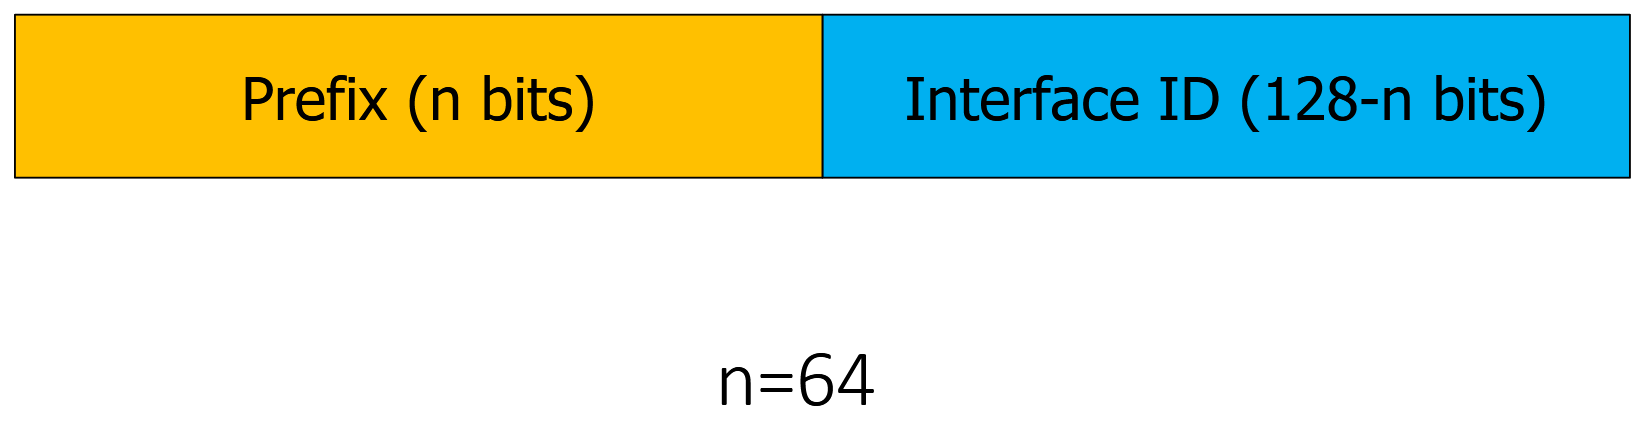
\includegraphics[width=0.6\textwidth]{capitoli/02-IPv6/images/ipv6_structure}
    \caption{Struttura dell'indirizzo IPv6 diviso tra Prefisso e Interface ID.}
    \label{fig:ipv6-struct}
\end{figure}

Una caratteristica distintiva (e per certi versi controintuitiva) di IPv6 è che lo standard suggerisce di fissare \textbf{sempre a 64 bit} la dimensione dell'Interface ID e, di conseguenza, a 64 bit la parte di Prefisso. Lo spazio è talmente vasto da permettere questo spreco per singola subnet.
Inoltre, non esistono le classi. Si mantiene la notazione CIDR \texttt{Indirizzo/N} per definire le aggregazioni nelle tabelle di routing (es. \texttt{FEDC:0123:8700::3/48}).

\section{Spazio di Indirizzamento e Tipologie di Indirizzi}

In IPv6 il concetto di \textit{broadcast} a livello di rete è stato completamente abolito, in quanto poco efficiente e sostituibile con meccanismi mirati. Esistono tre grandi famiglie di indirizzi: \textbf{Unicast}, \textbf{Multicast} e \textbf{Anycast}.

\subsection{Indirizzi Multicast}
Tutti gli indirizzi che iniziano con una sequenza di bit \texttt{1111 1111} (cioè \texttt{FF00::/8}) sono multicast. La struttura dell'indirizzo multicast comprende due campi di controllo fondamentali (Flag e Scope) prima del Group ID a 112 bit.
\begin{itemize}
    \item \textbf{T Flag:} Il bit "Transient" (0RPT). Se a 0, l'indirizzo è permanente (\textit{Well-known}, assegnato dalla IANA). Se a 1, è \textit{Transient} (assegnato dinamicamente, "che va e viene").
    \item \textbf{Scope (4 bit):} Definisce il raggio di propagazione del pacchetto. Il professore sottolinea l'importanza di questo campo: permette al router di sapere fin dove propagare il traffico senza fare flooding incontrollato. Ad esempio: \texttt{1} (Interface-local), \texttt{2} (Link-local), \texttt{5} (Site-local), \texttt{8} (Organization-local), \texttt{E} (Global). Lo streaming della cerimonia di ateneo, ad esempio, potrebbe essere limitato allo scope "Organization-local".
\end{itemize}

\begin{figure}[H]
    \centering
    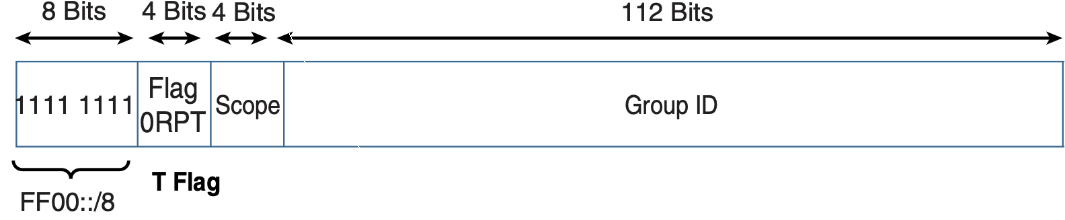
\includegraphics[width=0.5\textwidth]{capitoli/02-IPv6/images/ipv6_multicast_scope}
    \caption{Struttura dell'indirizzo Multicast IPv6: FF | T Flag | Scope | Group ID.}
    \label{fig:ipv6-multicast-scope}
\end{figure}

I principali blocchi multicast sono:
\begin{itemize}
    \item \textbf{Well-Known (\texttt{FF00::/12}):} Indirizzi predefiniti (es. "tutti i nodi sul link", "tutti i router").
    \item \textbf{Transient (\texttt{FF10::/12}):} Gruppi dinamici gestiti dalle applicazioni.
    \item \textbf{Solicited-Node (\texttt{FF02:0:0:0:0:1:FF00::/104}):} Di fondamentale importanza. Sostituisce il broadcast di livello IP usato storicamente per protocolli come ARP (per non disturbare tutte le macchine sulla rete locale, si invia a un gruppo specifico a cui si iscrive tendenzialmente un solo host).
\end{itemize}

\begin{figure}[H]
    \centering
    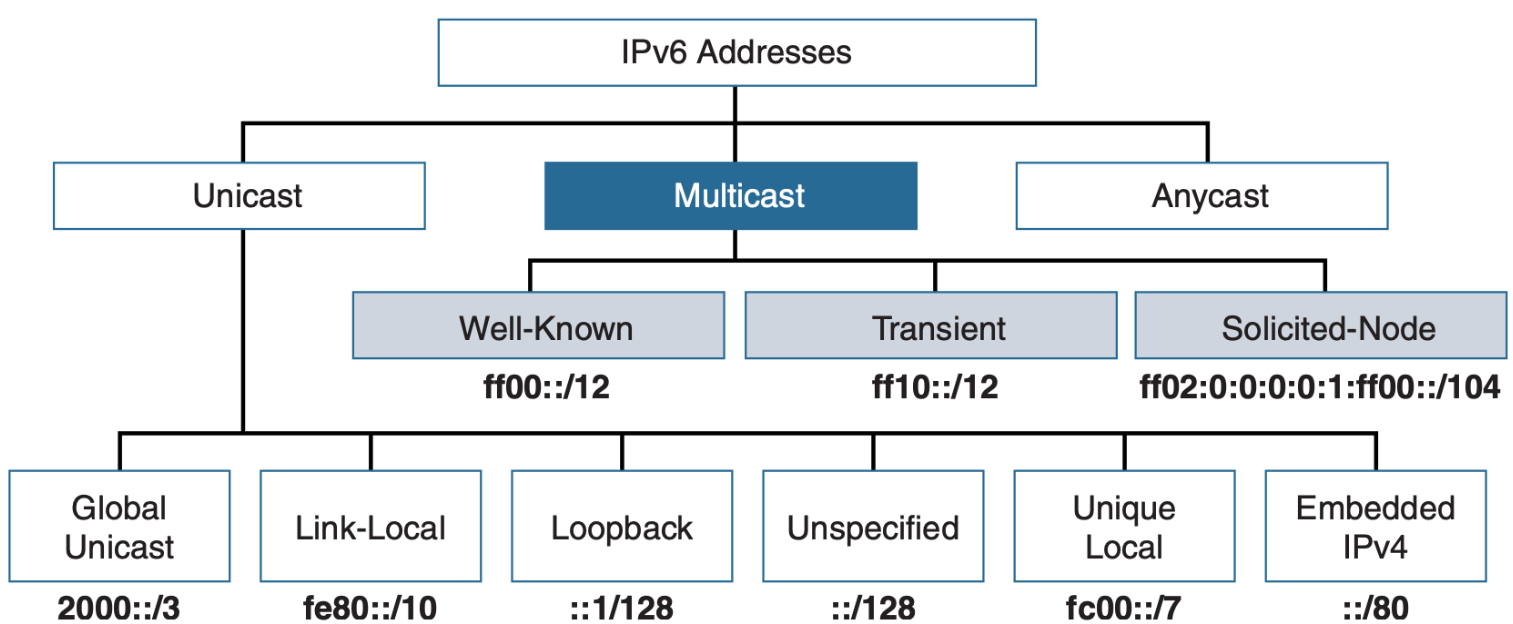
\includegraphics[width=0.7\textwidth]{capitoli/02-IPv6/images/ipv6_multicast_structure}
    \caption{Blocchi principali di indirizzi Multicast IPv6: Well-Known, Transient e Solicited-Node.}
    \label{fig:ipv6-multicast-structure}
\end{figure}

\subsection{Indirizzi Unicast}

\subsubsection{Global Unicast Addresses (\texttt{2000::/3})}
Rappresentano gli IP pubblici, instradabili globalmente. Iniziano tutti con la sequenza \texttt{001}.
Storicamente, si era pensato di dividere i primi 64 bit di prefisso in modo rigidamente gerarchico: TLA ID (Top-Level Authority, per i grandi provider), NLA ID (Next-Level Authority, per le organizzazioni) e SLA ID (Subnet Level Authority).
Successivamente, per garantire maggiore flessibilità, lo standard odierno divide i primi 64 bit semplicemente in due blocchi variabili:
\begin{enumerate}
    \item \textbf{Global Routing Prefix ($n$ bit):} Assegnato dal provider (ISP).
    \item \textbf{Subnet ID ($m$ bit):} Utilizzato dall'organizzazione per dividere la propria rete in sottoreti.
\end{enumerate}

\begin{figure}[H]
    \centering
    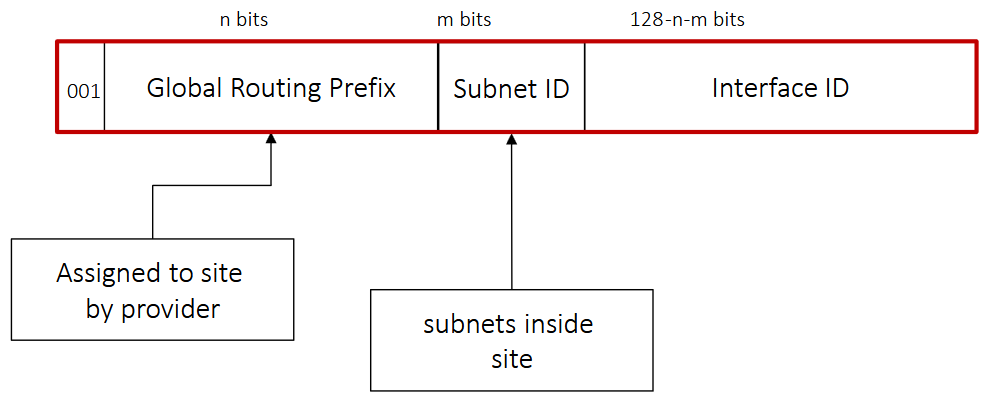
\includegraphics[width=0.7\textwidth]{capitoli/02-IPv6/images/ipv6_global_unicast}
    \caption{Struttura dell'indirizzo Global Unicast IPv6: Global Routing Prefix | Subnet ID | Interface ID.}
    \label{fig:ipv6-global-unicast}
\end{figure}

\subsubsection{Indirizzi Privati e Locali}
Così come in IPv4, vi è la necessità di indirizzi "privati".
\begin{itemize}
    \item \textbf{Link-Local (\texttt{FE80::/10}):} Hanno prefisso \texttt{1111 1110 10}. Sono validi unicamente all'interno della singola LAN fisica (il Link). Vengono usati pesantemente per l'autoconfigurazione e la Neighbor Discovery. I pacchetti destinati a questi IP non attraversano \textbf{mai} un router.
    \item \textbf{Site-Local (\texttt{FEC0::/10}):} Definiti originariamente ma ad oggi \textbf{deprecati} e sconsigliati.
    \item \textbf{Unique Local Addresses (ULA, \texttt{FC00::/7}):} Creati per l'uso privato, ma progettati per limitare i conflitti di instradamento in scenari aziendali complessi. Il prefisso operativo è di fatto \texttt{FD00::/8} (il flag L impostato a 1 indica assegnazione locale). Dopo i primi 8 bit, includono \textbf{40 bit generati pseudo-casualmente}, seguiti da 16 bit di Subnet ID e 64 bit di Interface ID. 
    \\ \textit{Osservazione del professore:} A cosa servono indirizzi privati generati in modo randomico? Se due sedi diverse di un'organizzazione (o due aziende che si fondono) usassero lo stesso prefisso privato (in IPv4 capita spessissimo con la classe \texttt{10.x.x.x}), collegandole in VPN vi sarebbe un conflitto di indirizzamento, risolvibile solo introducendo scomodi NAT intermedi. Con ULA, grazie ai 40 bit random, la probabilità di collisione è bassissima, consentendo l'instradamento diretto interno tra sedi (ma mai su Internet globale) senza bisogno di traduzione.
\end{itemize}

\subsubsection{Indirizzi Speciali}
\begin{itemize}
    \item \textbf{IPv4 Embedded (\texttt{::FFFF:x.y.w.z}):} Usati per la transizione, servono a rappresentare un nodo IPv4 all'interno di una rete IPv6 (gli ultimi 32 bit ospitano l'indirizzo IPv4, con notazione puntata convenzionale).
    \item \textbf{Loopback (\texttt{::1/128}):} L'equivalente di \texttt{127.0.0.1}. Usato per test locali.
    \item \textbf{Unspecified (\texttt{::/128}):} Sequenza di soli zeri. Usato come indirizzo sorgente in specifici pacchetti (come la Duplicate Address Detection) per indicare che l'interfaccia non ha ancora acquisito un IP valido.
\end{itemize}

\begin{figure}[H]
    \centering
    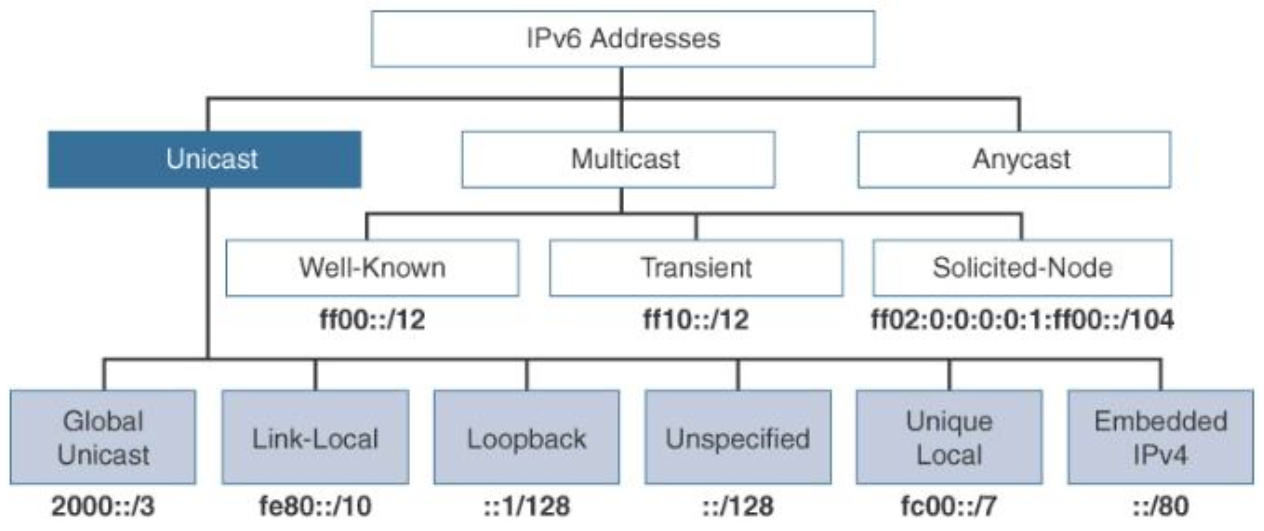
\includegraphics[width=0.7\textwidth]{capitoli/02-IPv6/images/ipv6_addresses}
    \caption{Tipologie di indirizzi IPv6 unicast.}
    \label{fig:ipv6-special-addresses}
\end{figure}

\subsection{Indirizzi Anycast}
Gli indirizzi Anycast sfruttano lo spazio di indirizzamento dei Global Unicast, ma violano la regola per cui un IP identifica unicamente un'interfaccia.
Un indirizzo Anycast viene assegnato a \textbf{più dispositivi} geograficamente distribuiti. Quando un utente contatta quell'IP, i protocolli di routing standard (scegliendo la "shortest path") instradano il pacchetto verso la replica del server topologicamente "più vicina".
Il professore cita il caso dei server DNS pubblici (es. i DNS di Google). In IPv4 l'IP \texttt{8.8.8.8} risiede su decine di datacenter nel mondo; analogamente, i corrispettivi IPv6 (es. \texttt{2001:4860:4860::8888}) sono Anycast. L'enorme vantaggio di Anycast è che non richiede alcuna logica speciale: si basa sul naturale funzionamento del routing. Le reti CDN (Content Delivery Network) ne fanno ampio uso.

\section{Modifiche all'Architettura dei Protocolli}

L'introduzione di IPv6 provoca una "reazione a catena" nell'architettura di rete, confutando l'idea di una rigida indipendenza tra livelli (\textit{Layer Independence}). IPv4 non è facilmente sostituibile perché protocolli di livello superiore e inferiore dipendono dal suo formato:
\begin{itemize}
    \item \textbf{ICMP} viene esteso e diventa \textbf{ICMPv6}.
    \item Protocolli come \textbf{ARP} (scoperta dei MAC) e \textbf{IGMP} (gestione multicast) vengono eliminati come entità separate e \textbf{le loro funzioni sono interamente assorbite da ICMPv6}.
    \item \textbf{DNS} necessita di un nuovo record: i record tipo \texttt{A} mantengono la mappatura nomi-IPv4, mentre vengono introdotti i record tipo \textbf{\texttt{AAAA}} per mappare nomi-IPv6.
    \item \textbf{I protocolli di routing} (BGP, OSPF, RIP) vanno aggiornati per gestire prefissi su 128 bit.
    \item \textbf{Socket Interface:} I software applicativi, scritti usando le socket TCP/UDP, devono essere riprogrammati o aggiornati per passare al sistema operativo IP sorgente e destinazione su 128 bit.
\end{itemize}

\section{Formato del Pacchetto (Header IPv6)}

La transizione da 32 a 128 bit per gli indirizzi introduce un sovraccarico per le CPU e l'hardware dedicato dei router di backbone. Per compensare, \textbf{l'header IPv6 è stato fortemente snellito e reso a dimensione fissa (40 byte)}.

% FIGURA ORIGINALE DA RECUPERARE DALLE SLIDE
% Slide di provenienza: "IPv4 Header" e "IPv6 Header"
% Tipo: Tabella comparativa (schema)
% Descrizione: Confronto visivo tra l'header IPv4 (complesso e a lunghezza variabile) e IPv6 (snello a 40 byte fissi).
% Punto di inserimento: Inizio sezione Header IPv6.
\begin{figure}[H]
    \centering
    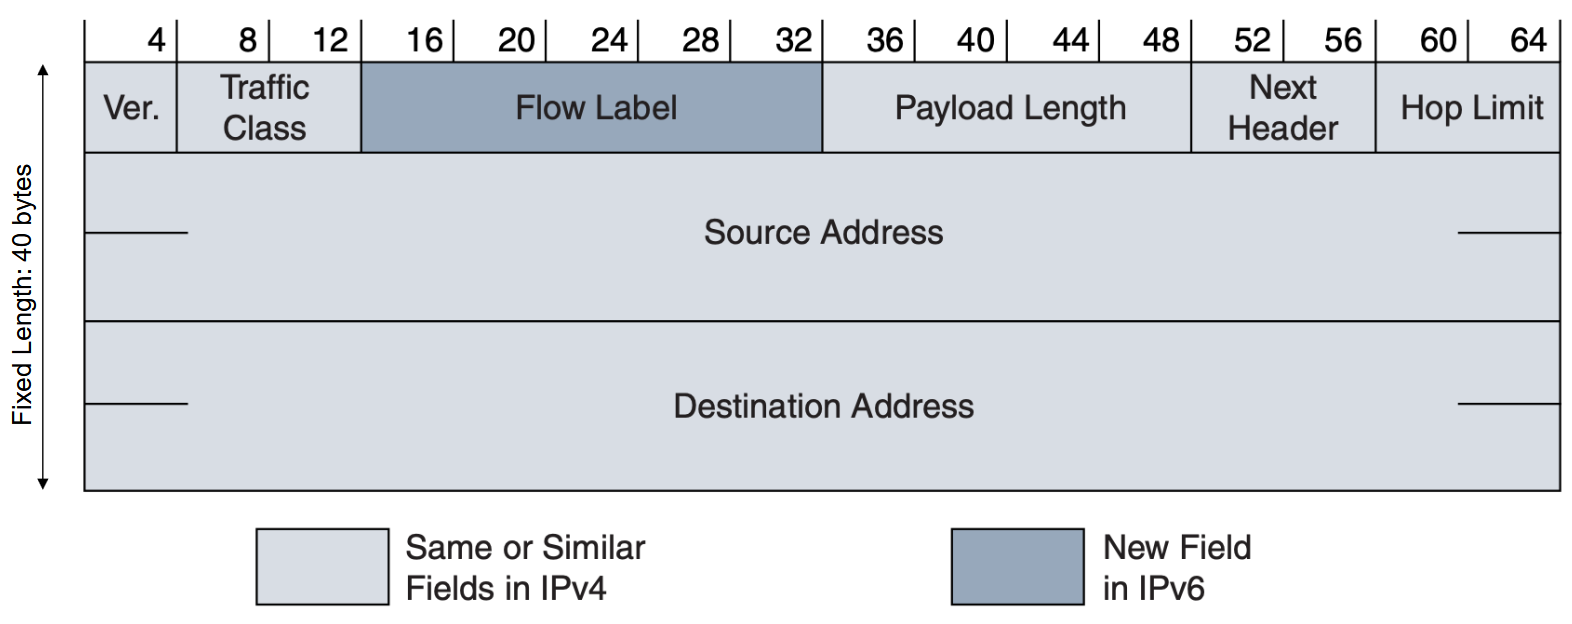
\includegraphics[width=0.85\textwidth]{capitoli/02-IPv6/images/ipv6_header}
    \caption{L'Header IPv6, semplificato e di dimensione fissa (40 byte).}
    \label{fig:ipv6-header}
\end{figure}

\subsection{Campi Eliminati rispetto a IPv4}
\begin{itemize}
    \item \textbf{Header Length:} Rimosso poiché la lunghezza è ora fissa (40 byte). Le opzioni vengono gestite diversamente.
    \item \textbf{Header Checksum:} Rimosso poiché ridondante. Il calcolo della correttezza dei bit viene già effettuato al livello 2 (es. FCS in Ethernet) e al livello 4 (la checksum del TCP o dell'UDP, che per IPv6 diventa obbligatoria e copre anche parti dell'header IP tramite lo \textit{pseudo-header}). Evitare il calcolo della checksum a ogni hop alleggerisce notevolmente i router.
    \item \textbf{Fragment Offset, Identification, Flags (Frammentazione):} I router IPv6 \textbf{non frammentano più i pacchetti in transito}. Se un router riceve un pacchetto più grande della MTU del link di uscita (es. pacchetto da 4096 byte su link da 2048 byte), scarta il pacchetto e invia al mittente un messaggio d'errore ICMPv6 "Packet Too Big". Sarà il mittente (l'host) a ricalibrare la dimensione e frammentare i dati a livello sorgente o applicativo (Path MTU Discovery). Questo elimina ai router il gravoso compito della frammentazione.
\end{itemize}

\subsection{Campi Presenti (Mantenuti o Rinominati)}
\begin{itemize}
    \item \textbf{Version (4 bit):} Vale 6 (0110).
    \item \textbf{Traffic Class (8 bit):} Precedentemente \textit{Type of Service (ToS)} o \textit{DiffServ}. Usato dagli operatori per classificare il traffico (es. per dare priorità a un flusso video su una mail).
    \item \textbf{Payload Length (16 bit):} Sostituisce il \textit{Total Length}. Indica i byte successivi ai 40 byte di header IP.
    \item \textbf{Next Header (8 bit):} Sostituisce il campo \textit{Protocol}. Indica cosa si trova immediatamente dopo l'header IPv6 (es. TCP, UDP, ICMPv6 o un Extension Header).
    \item \textbf{Hop Limit (8 bit):} Rinominazione del \textit{Time To Live (TTL)}. Viene decrementato di 1 a ogni router per prevenire loop infiniti in rete.
    \item \textbf{Source e Destination Address:} Passati a 128 bit.
\end{itemize}

\subsection{La Novità: Il campo Flow Label (20 bit)}
In IPv4, l'hardware di rete per identificare a quale "flusso" o sessione appartenesse un pacchetto (magari per applicare regole di prioritizzazione o policy routing) estraeva la cosiddetta \textbf{Quintupla (5-tuple)}: IP sorgente, IP destinazione, Porta sorgente, Porta destinazione, Protocollo. Estrarre le porte significa fare \textit{cross-layering} (dover ispezionare il livello Trasporto).
Per evitare questo, in IPv6 la sorgente può assegnare a un pacchetto un'etichetta univoca di 20 bit, il \textbf{Flow Label} (es. flusso mail = 001, flusso video = 002). I router intermedi potranno instradare e applicare regole guardando unicamente IP sorgente e Flow Label, aumentando drasticamente l'efficienza.

\subsection{Gli Extension Headers (Chaining)}
Poiché la lunghezza base è fissa, le opzioni aggiuntive vengono agganciate in "cascata" (chaining) sfruttando il campo \textbf{Next Header}.
Se il pacchetto base prevede un'opzione, il campo Next Header indicherà il codice di quell'estensione. L'estensione, a sua volta, avrà il suo campo Next Header per indicare cosa segue (TCP, UDP, o un'altra estensione).

% FIGURA ORIGINALE DA RECUPERARE DALLE SLIDE
% Slide di provenienza: "Header Chaining"
% Tipo: Diagramma a blocchi
% Descrizione: Rappresentazione visiva di come i Next Header puntano al blocco successivo (IPv6 Header -> Extension Header -> TCP Header).
% Punto di inserimento: Spiegazione Extension Headers.
\begin{figure}[H]
    \centering
    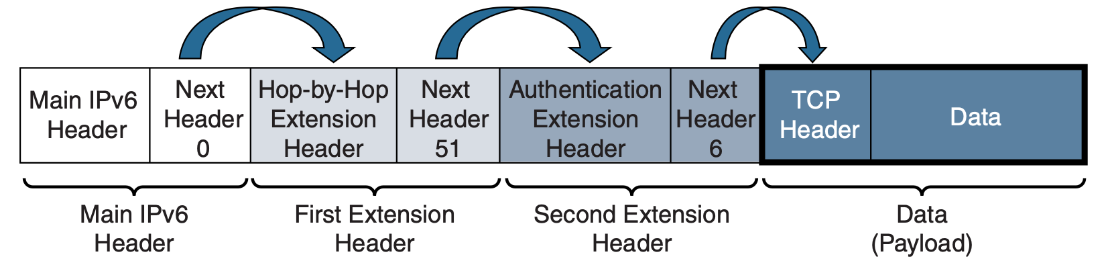
\includegraphics[width=0.7\textwidth]{capitoli/02-IPv6/images/header_chaining}
    \caption{Meccanismo di concatenamento (chaining) degli Extension Headers.}
    \label{fig:header-chain}
\end{figure}

Gli header di estensione più rilevanti sono:
\begin{itemize}
    \item \textbf{Hop-by-Hop Option (0):} Informazioni che devono essere elaborate da \textbf{ogni singolo router} lungo il percorso. Contiene opzioni in formato TLV (Type, Length, Value). Il professore fa l'esempio di un pacchetto di telemedicina per cui si inserisce un "timestamp", ordinando ai router di scartare il dato se sono passati più di 0.5 secondi. Grazie al TLV, se un router non riconosce l'opzione (Type), non scarta il pacchetto ma semplicemente la ignora. Contiene anche l'opzione \textit{Jumbogram} (per payload > 65.535 byte, tipici dei Datacenter).
    \item \textbf{Fragment Header (44):} Utilizzato solo se l'host sorgente ha reale necessità di inviare pacchetti frammentati.
    \item \textbf{Routing Extension (43):} Utilizzato per forzare un percorso specifico (\textit{Source routing}).
    \item \textbf{IPsec (AH 51, ESP 50):} Permette l'implementazione della sicurezza nativa (Authentication Header per l'integrità, Encapsulating Security Payload per la cifratura).
\end{itemize}

\section{Interfacciamento con il Livello Data Link}

Quando un pacchetto IPv6 viene incapsulato in una trama Ethernet, il campo EtherType (Type a livello MAC) assume il valore \texttt{0x86DD}. Trattare IPv6 come un nuovo protocollo separato da IPv4 (\texttt{0x0800}) permette il funzionamento in \textit{Dual Stack} sulla stessa rete fisica.

\subsection{Indirizzamento Multicast a livello MAC}
Poiché i frame di broadcast inquinano la rete (costringendo tutte le NIC, Network Interface Card, a processarli passandoli alla CPU), IPv6 si basa sul multicast Ethernet.
C'è una mappatura algoritmica standard (RFC 7042): l'indirizzo MAC di destinazione per un pacchetto IPv6 Multicast inizia sempre con il prefisso \texttt{33:33}, seguito dagli ultimi 32 bit (4 byte) dell'indirizzo IPv6 multicast.

Esempio fornito nelle slide:
Se l'indirizzo IPv6 Multicast è \texttt{FF0C::89:AABB:CCDD}, gli ultimi 32 bit sono \texttt{AA:BB:CC:DD}.
L'indirizzo MAC sarà \texttt{33:33:AA:BB:CC:DD}.

Le schede di rete (NIC) vengono programmate (via driver) per intercettare e far passare solo i frame MAC che corrispondono ai gruppi multicast a cui l'host è iscritto. Questo risolve l'efficienza sulle LAN.

\section{ICMPv6 e Neighbor Discovery}

Il protocollo ICMPv6 è vitale per IPv6 (viene trasportato con Next Header = 58) e si fa carico di numerosissime funzioni:
\begin{itemize}
    \item \textbf{Messaggi di errore:} Destination Unreachable (Tipo 1), Packet too big (Tipo 2, fondamentale per la MTU discovery senza frammentazione nei router), Time exceeded (Tipo 3, TTL=0), Parameter Problem (Tipo 4).
    \item \textbf{Messaggi informazionali (Echo):} Echo Request (128) ed Echo Reply (129), la base del comando \texttt{ping}.
\end{itemize}

\subsection{Sostituzione di ARP: Neighbor Solicitation e Advertisement}
In IPv4, il protocollo ARP inviava un messaggio broadcast MAC (\texttt{FF:FF:FF:FF:FF:FF}) per ottenere il MAC address associato a un IP target.
In IPv6, ARP è rimosso e sostituito dalla \textbf{Neighbor Discovery (ND)}.

% FIGURA ORIGINALE DA RECUPERARE DALLE SLIDE
% Slide di provenienza: "Address Resolution"
% Tipo: Diagramma di sequenza / Schema
% Descrizione: Funzionamento dello scambio ICMP tra Requester (Neighbor Solicitation) e il nodo che risponde (Neighbor Advertisement).
% Punto di inserimento: Spiegazione Address Resolution.
\begin{figure}[H]
    \centering
    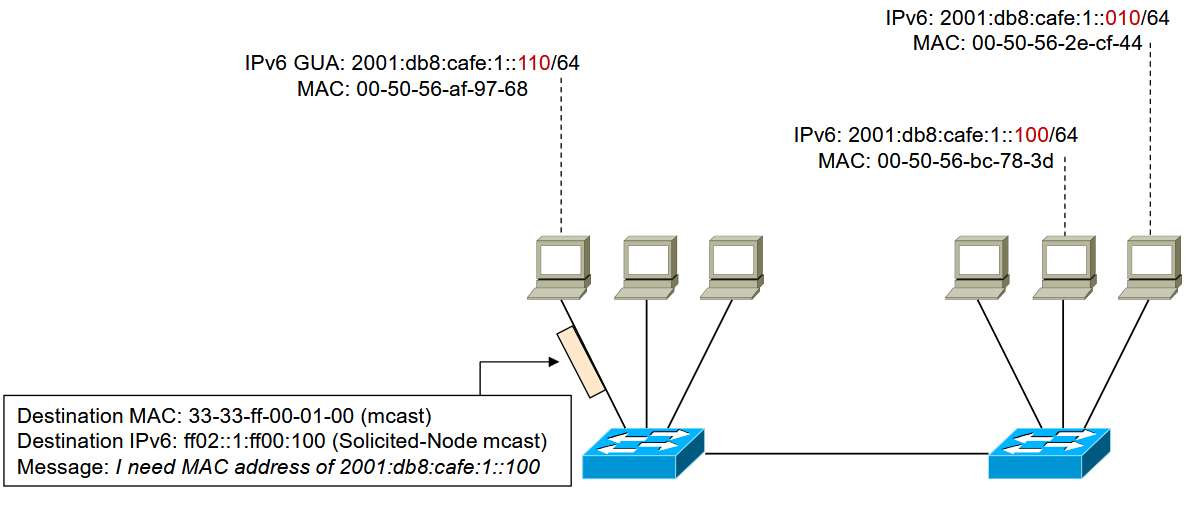
\includegraphics[width=0.6\textwidth]{capitoli/02-IPv6/images/nd_resolution}
    \caption{Processo di risoluzione degli indirizzi (Address Resolution) tramite Neighbor Solicitation.}
    \label{fig:nd-res}
\end{figure}

Il meccanismo sfrutta il \textbf{Solicited-Node Multicast Address}:
Quando un'interfaccia acquisisce un indirizzo unicast, calcola e si iscrive automaticamente a un gruppo multicast formato dal prefisso fisso \texttt{FF02:0:0:0:0:1:FF00::/104} concatenato ai \textbf{24 bit meno significativi} del proprio IP.
Perché fare questo? Quando il Nodo A vuole scoprire il MAC del Nodo B:
\begin{enumerate}
    \item Crea un pacchetto \textbf{Neighbor Solicitation (Tipo 135)}. Nel payload c'è l'IP target di cui cerca il MAC.
    \item L'IP destinazione non è un broadcast, ma il \textit{Solicited-Node Multicast} calcolato a partire dall'IP target.
    \item Il pacchetto viene inviato al corrispondente indirizzo MAC Multicast (es. \texttt{33:33:FF:XX:XX:XX}).
\end{enumerate}
In questo modo, lo switch inoltrerà il frame, ma \textbf{solo le interfacce i cui ultimi 24 bit dell'IP coincidono con quelli ricercati riceveranno il frame a livello hardware}. Statisticamente, riceverà il pacchetto unicamente il nodo target, il quale risponderà con un \textbf{Neighbor Advertisement (Tipo 136)}. 

\subsection{Sostituzione di IGMP: Multicast Group Management}
La gestione dei gruppi multicast, in IPv4 affidata al protocollo a sé stante IGMP, rientra ora tra i tipi di ICMPv6. I messaggi essenziali per permettere ai router di sapere a quali flussi i client della subnet sono iscritti sono:
\begin{itemize}
    \item \textbf{Multicast Listener Query (130):} Il router interroga la rete.
    \item \textbf{Multicast Listener Report (131):} Un host notifica di volersi unire a un gruppo.
    \item \textbf{Multicast Listener Done (132):} L'host esce dal gruppo.
\end{itemize}

\section{Autoconfigurazione dei Dispositivi}

IPv6 nasce con l'ambizione del \textit{plug-and-play} nativo tramite \textbf{SLAAC (Stateless Address Autoconfiguration)}, riducendo la necessità di server DHCP centralizzati.
Per operare, un host ha bisogno di due informazioni primarie:
\begin{enumerate}
    \item Generare la parte host (Interface ID, 64 bit).
    \item Ottenere la parte di rete (Prefix, 64 bit).
\end{enumerate}

\subsection{Generazione dell'Interface ID}
L'approccio storico si basava sul formato \textbf{EUI-64}, partendo dal MAC Address a 48 bit della scheda:
\begin{enumerate}
    \item Si divide in due il MAC address (da 24 bit ciascuna).
    \item Si inietta nel mezzo la sequenza esadecimale \texttt{FFFE}.
    \item \textbf{Gestione dello "Universal Bit":} Il settimo bit del primo byte del MAC indica se è amministrato localmente (1) o universalmente (0). In IPv6 la convenzione è invertita: un IP è identificato univocamente in modo globale se il settimo bit è a \textbf{1}. Quindi, il settimo bit del MAC Address generato viene "flippato" (invertito) nel passaggio a Interface ID. (Nota: Se in futuro si useranno MAC nativi a 64 bit, il processo di iniezione di \texttt{FFFE} decadrà).
\end{enumerate}

\begin{figure}[H]
    \centering
    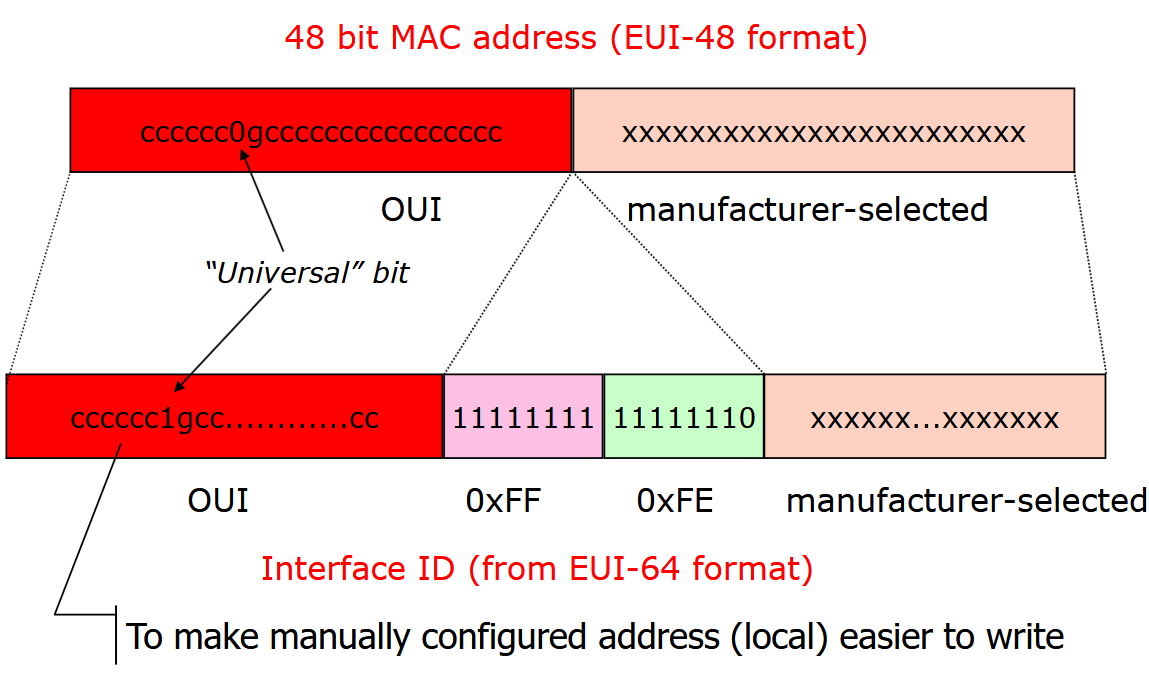
\includegraphics[width=0.7\textwidth]{capitoli/02-IPv6/images/eui64}
    \caption{Generazione dell'Interface ID a partire dal MAC Address secondo lo standard EUI-64.}
    \label{fig:eui64}
\end{figure}

\textbf{Privacy concerns e Indirizzi Random (Privacy Extensions RFC 4941):}
Se l'Interface ID è derivato dal MAC, la parte finale dell'IP dell'host rimane costante ovunque egli si trovi (a casa, in università, in aeroporto). Un osservatore malevolo potrebbe tracciarne gli spostamenti incrociando i log dei server web.
Per impedirlo, lo standard suggerisce un \textbf{Privacy Extension Algorithm}:
L'Interface ID si genera calcolando l'hash MD5 di (Indirizzo Random a 64 bit precedentemente usato concatenato al MAC originario). Se ne prendono i primi 64 bit, assicurandosi di impostare a 0 il settimo bit (\textit{Universal bit}) tramite un'operazione \texttt{AND bit-a-bit} con una maschera.
A ogni nuova associazione l'hash garantisce che l'IP sia sempre diverso e non riconducibile all'hardware fisico.
I moderni OS mantengono due indirizzi: uno derivato staticamente e uno "privacy-aware" per le connessioni in uscita.

\begin{figure}[H]
    \centering
    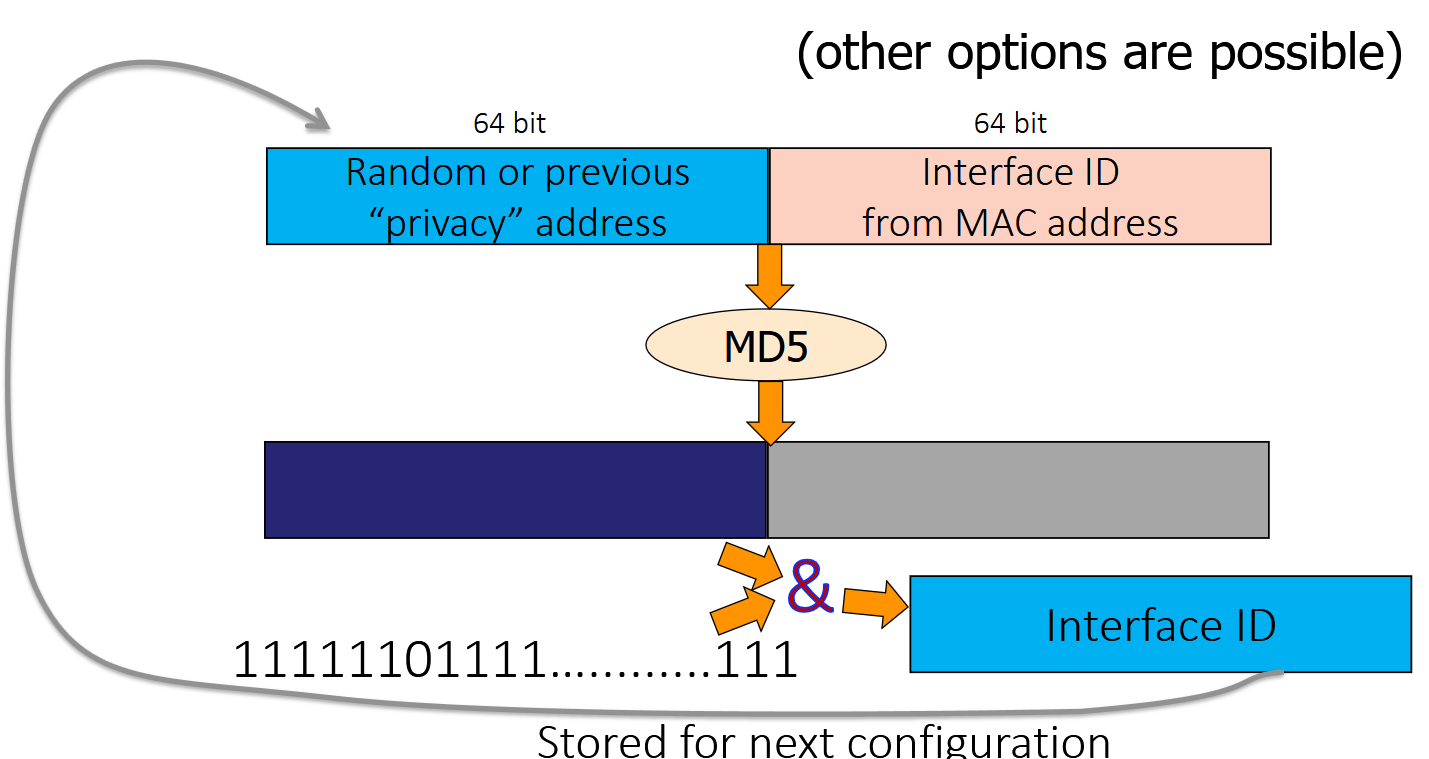
\includegraphics[width=0.7\textwidth]{capitoli/02-IPv6/images/privacy_extension}
    \caption{Generazione dell'Interface ID con Privacy Extension (RFC 4941).}
    \label{fig:privacy-extension}
\end{figure}

\subsection{Ottenimento del Prefisso (Router Discovery)}
Mentre l'Interface ID è autogenerato, il prefisso di rete (\texttt{Prefix/64}) deve essere fornito dal router per indirizzi globali. Un host privo di prefisso instradabile può solo autoconfigurarsi un IP Link-Local (generando l'interface ID e accodandolo al prefisso standard \texttt{FE80::}).
Per ottenere un Global Unicast si utilizzano messaggi ICMPv6:
\begin{enumerate}
    \item \textbf{Router Solicitation (RS - Tipo 133):} Inviato dall'host all'accensione verso l'indirizzo multicast \texttt{FF02::2} (Tutti i router).
    
    \begin{figure}[H]
        \centering
        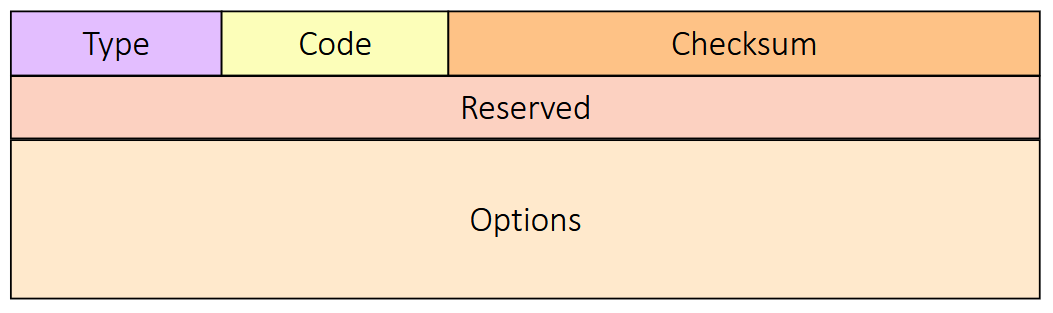
\includegraphics[width=0.7\textwidth]{capitoli/02-IPv6/images/router_solicitation}
        \caption{Messaggio di Router Solicitation (RS).}
        \label{fig:router-solicitation}
    \end{figure}

    \item \textbf{Router Advertisement (RA - Tipo 134):} I router rispondono (o inviano periodicamente) questo pacchetto. All'interno si trovano opzioni fondamentali formulate in blocchi TLV.

    \begin{figure}[H]
        \centering
        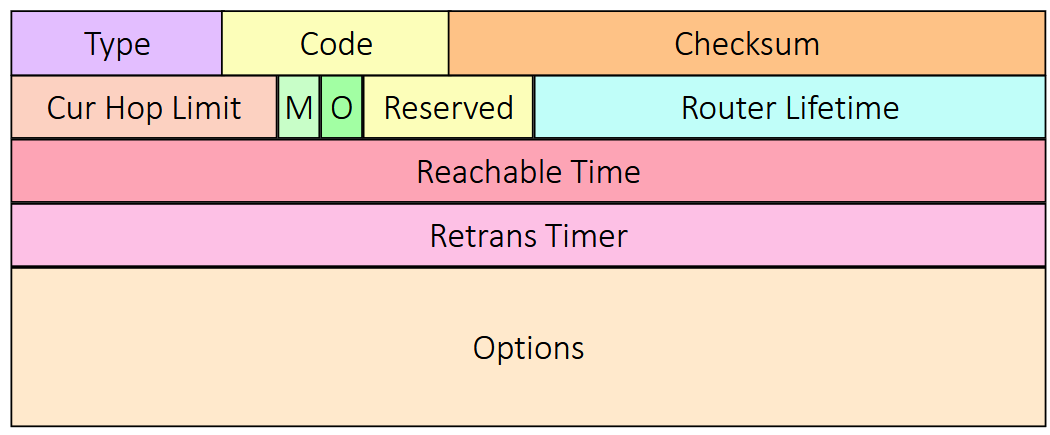
\includegraphics[width=0.7\textwidth]{capitoli/02-IPv6/images/router_advertisement}
        \caption{Messaggio di Router Advertisement (RA).}
        \label{fig:router-advertisement}
    \end{figure}

\end{enumerate}

Un Router Advertisement contiene dei flag per indicare alla macchina dove recuperare le informazioni non presenti nell'header base:
\begin{itemize}
    \item \textbf{M (Managed):} Se 1, segnala che un server DHCPv6 è presente per gestire lo stateful address configuration.
    \item \textbf{O (Other):} Se 1, segnala di contattare il DHCP per informazioni ausiliarie (come il server DNS).
\end{itemize}

Tra le opzioni (Options) dell'RA, il router invia:
\begin{itemize}
    \item \textbf{Prefix Information:} Comunica il \texttt{Prefisso/64} da usare per comporre l'IP. Tramite flag (\textit{A - Autonomous}) il router autorizza l'host a usare questo prefisso per l'autoconfigurazione SLAAC. Se non è flaggato, l'host usa l'IP per crearsi le routing table, ma necessita del DHCP per un IP.
    
    \begin{figure}[H]
        \centering
        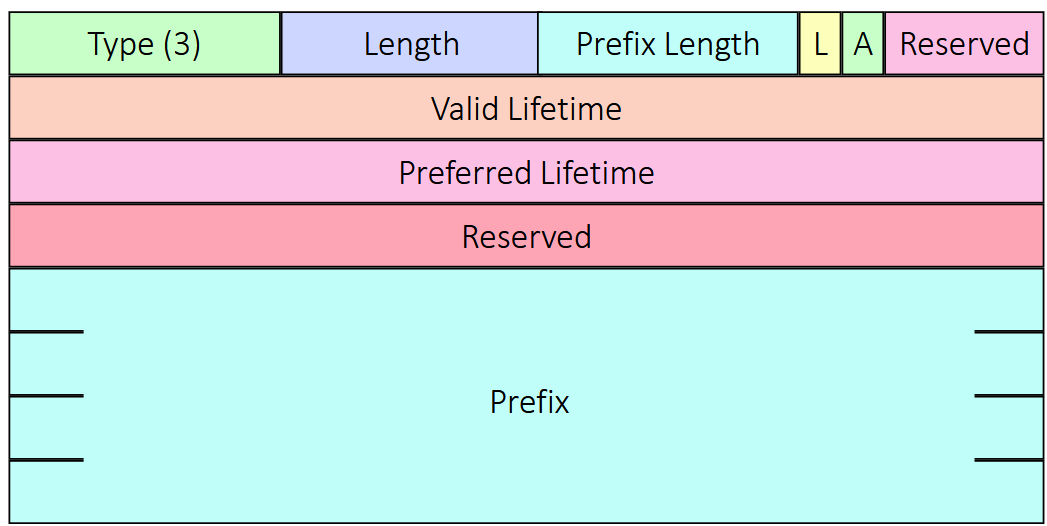
\includegraphics[width=0.7\textwidth]{capitoli/02-IPv6/images/prefix_information}
        \caption{Opzione "Prefix Information" all'interno del Router Advertisement.}
        \label{fig:prefix-information}
    \end{figure}

    \item \textbf{MTU Option:} La massima dimensione del pacchetto sulla rete fisica locale.
    
    \begin{figure}[H]
        \centering
        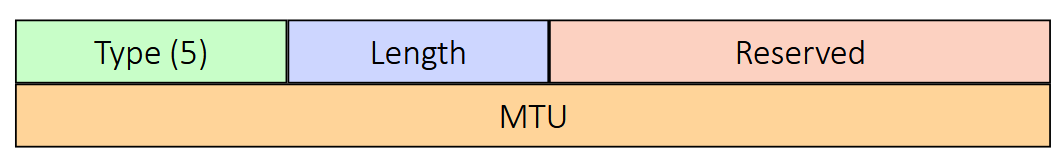
\includegraphics[width=0.7\textwidth]{capitoli/02-IPv6/images/mtu_option}
        \caption{Opzione "MTU" all'interno del Router Advertisement.}
        \label{fig:mtu-option}
    \end{figure}
    
    \item \textbf{Link Layer Address:} Spesso il router include il suo stesso MAC Address, risparmiando all'host di dover fare una successiva Neighbor Solicitation per cercare il gateway di uscita su Internet.

    \begin{figure}[H]
        \centering
        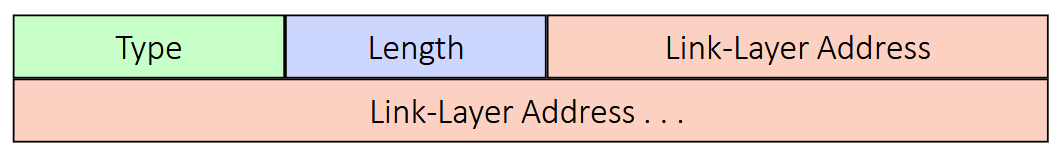
\includegraphics[width=0.7\textwidth]{capitoli/02-IPv6/images/link_layer_address}
        \caption{Opzione "Link Layer Address" all'interno del Router Advertisement.}
        \label{fig:link-layer-address}
    \end{figure}

\end{itemize}

\subsection{ICMP Redirect (Ottimizzazione First Hop)}
Il pacchetto \textbf{Redirect (Tipo 137)} interviene in LAN con più router (es. R1 e R2). Se l'host usa di default R1 per raggiungere una rete esterna, ma R1 si accorge (tramite tabelle di routing interne) che per quella specifica destinazione R2 è topologicamente più appropriato, R1 inoltra la prima richiesta e parallelamente invia un messaggio "Redirect" all'host. R1 dice: "Per il target X, il gateway ottimale non sono io, ma R2". Questo vale solo per la scelta a livello locale (First Hop).

\begin{figure}[H]
    \centering
    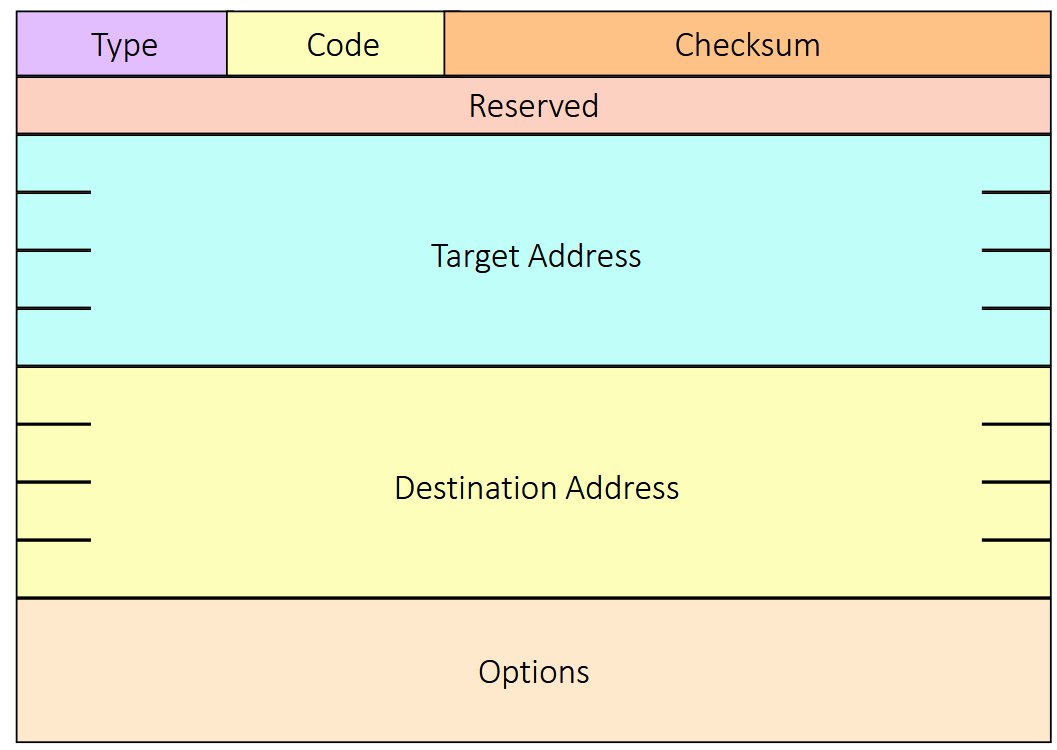
\includegraphics[width=0.7\textwidth]{capitoli/02-IPv6/images/icmp_redirect}
    \caption{Formato del messaggio ICMP Redirect: Reserved, Target Address, Options e Destination Address.}
    \label{fig:icmp-redirect}
\end{figure}

\subsection{Duplicate Address Detection (DAD)}
Sia che l'host componga il suo indirizzo con il MAC mapping, sia con l'algoritmo pseudo-casuale, \textbf{la certezza assoluta dell'univocità non esiste}. Prima di utilizzare l'indirizzo (anche il Link-Local), il nodo deve provare che non ci siano conflitti eseguendo la \textbf{DAD}.
Procedura:
\begin{enumerate}
    \item L'host forma l'IP desiderato (es. Link-Local \texttt{FE80::1A2B}).
    \item Invia una \textbf{Neighbor Solicitation (NS)} interrogando la rete per l'IP appena formato.
    \item Il campo \textbf{Source Address del pacchetto IP è impostato a Unspecified (\texttt{::})}, perché l'host non ha ancora formalmente l'autorizzazione a usare l'IP. L'indirizzo di destinazione è il \textit{Solicited-Node Multicast Address} corrispondente.
    \item Se entro $\sim 1$ secondo \textbf{nessuno risponde} con un \textit{Neighbor Advertisement (NA)}, il silenzio vale come conferma. L'indirizzo è libero e il nodo lo acquisisce. Se riceve un NA, c'è una collisione e l'host deve ricalcolare l'ID (es. richiamando l'MD5 o fallendo il setup).
\end{enumerate}
Subito dopo aver superato la DAD, il nodo iscrive il MAC alla NIC e invia formale notifica di iscrizione al gruppo (Multicast Listener Report). Come fa notare il docente: essendo il \textit{Solicited-Node} generato in base agli ultimi 24 bit, statisticamente l'host in questione sarà l'unico iscritto a tale gruppo su quel link. L'invio del \textit{Report} è concettualmente superfluo in tal caso, ma viene eseguito per consistenza dell'implementazione del software dei sistemi operativi.

\subsection{Indirizzi con Scope (Scoped Addresses)}
Poiché ogni interfaccia fisica auto-genera un indirizzo Link-Local (con prefisso identico \texttt{FE80::}), una macchina (es. un router) dotata di molte interfacce avrebbe diversi IP che sembrano afferire alla medesima sottorete, pur mappando su link fisici differenti.
A livello del sistema operativo (es. interfacce a riga di comando Linux/Windows), l'ambiguità viene risolta aggiungendo lo \textbf{Scope ID} in fondo all'IP, separato dal simbolo \texttt{\%}. Questo numero indica banalmente l'indice dell'interfaccia.
Esempio: \texttt{FE80::0237:00FF:FE02:A7FD\%19} (L'indirizzo sull'interfaccia fisica numero 19).

\begin{figure}[H]
    \centering
    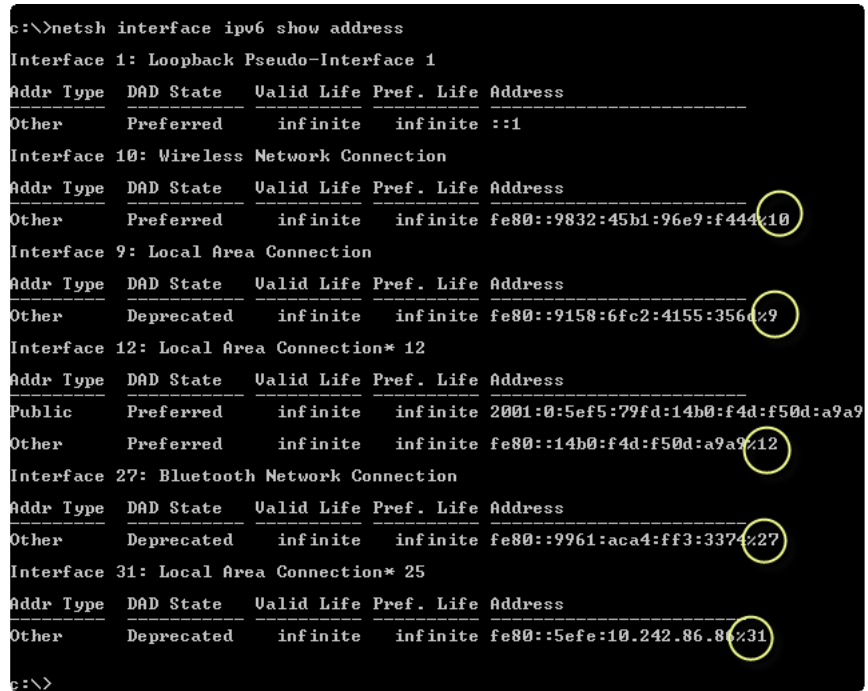
\includegraphics[width=0.7\textwidth]{capitoli/02-IPv6/images/scoped_address}
    \caption{Esempio di indirizzo IPv6 con Scope ID per risolvere ambiguità tra interfacce.}
    \label{fig:scoped-address}
\end{figure}